\chapter{A Data Perspective to Scalable Learning}
\label{ch:data}

We now turn our attention to scalably learning a PC purely from data. In this chapter, we look at
PCs solely from the perspective of data fitness; we exploit the connection between PCs and
generative random forests \citep{correia20,ho95} and revisit a well-known technique based on random
projections for constructing random trees \citep{dasgupta08a,dasgupta08b}, presenting a simple and
fast yet effective way of learning PCs. This approach learns smooth and structured decomposable
circuits by randomly partitioning the data space with random projections in a \divclass{} class
fashion. We show that our method produces competitive PCs at a fraction of the time. The
contributions in this chapter come, in part, from \citet{geh21b}.

\section{Probabilistic Circuits and Decision Trees}
\label{sec:data}

Before we go through with our proposal in detail, we must first lay the groundwork and motivate the
decisions behind our structure learning algorithm. We begin by re-emphasizing the connection
between probabilistic circuits and density estimation trees briefly discussed in \Cref{eg:det}. We
follow by revisiting \emph{random projections} \citep{dasgupta08a,dasgupta08b}, a well-known
technique for hierarchically partitioning data through oblique hyperplanes. Next, we present in
detail a very fast structure learning algorithm for quickly generating smooth and structured
decomposable circuits. Despite their simplicity, we empirically show their competitive performance
compared to state-of-the-art.

Recently, \citet{correia20} showed that (ensembles of) decision trees (DTs) learned for prediction
tasks can be easily extended into full probabilistic models represented as probabilistic circuits.
Besides equipping decision forests with more principled approaches to handling missing data and
diagnosing outliers, this bridge between decision trees and PCs suggests an interesting alternative
to learning the latter using the efficient inductive algorithms available for the former
\citep{correia20,ram11,khosravi20}. Despite this, most works addressing such a connection have
focused on the discriminative side of DTs, with much of the effort put onto classification rather
than generative tasks such as density estimation. Here, we explore the generative side of DTs,
often referred as density estimation trees (DETs, \cite{ram11,hang19,smyth95}), within the framework
of PCs, taking inspiration from known algorithms for building DTs and DETs, and transplanting them
to PCs.

As only shortly discussed in \Cref{eg:det}, yet better formalized by \citet{correia20}, a DET can
be represented as a smooth and deterministic tree-shaped PC with only sums and input nodes by
interpreting sum nodes as latent variables describing the partitioning of data, and making sure
that the supports of input nodes are restricted to the data cells induced by all the partitionings
done by the sums. The resulting density of this DET PC is given by
\begin{equation}
  p_\mathcal{C}(\set{x})=\sum_{\Leaf\in\operatorname{Inputs}(\mathcal{C})}w_{\Leaf}\cdot\Leaf(\set{x})\cdot\liv\set{x}\in\Leaf\riv,
\end{equation}
where $\liv\set{x}\in\Leaf\riv$ is an indicator function that returns 1 if $\set{x}$ is within
$\Leaf$'s cell and 0 otherwise. The above formula comes from collapsing a circuit with only sum
layers, where each sum corresponds to a latent variable representing a partitioning of the data,
into a single-layer shallow PC. These latent variables usually consist of partitioning data through
hyperplanes, dividing data into two parts, each represented as the subcircuit rooted at each child
of the sum node.

A $k$-d tree is a subclass of decision trees which hierarchically partitions data into more or less
equally sized parts, usually by splitting the data according to the value of a single variable at a
time \citep{bentley75,hang19,ho95}, essentially producing axis-aligned hyperplanes.
\citet{dasgupta08b} noted that such an approach cannot ensure that the resulting partitioning of
the input space approximates the intrinsic dimensionality of data (roughly understood as a manifold
of low dimension). In contrast, they provide a simple strategy for space partitioning that consists
in recursively partitioning the space according to a random separating hyperplane. This
approximates a random projection of the data and has the following theoretical guarantee
\citep{dasgupta08b}:

\begin{figure}[t]
  \def\points{(2.3,4.38),(1.8,4.0),(2.8,4.0),(1.6,3.3),(2.5,3),(3.1,2.8),(3.8,3.1),(4.3,3.3),(4,2.6),(4.5,2.4),(3.3,2.3),(2.1,2.0),(3.1,1.8),(2.4,1.6),(2.9,1.5),(2.5,1.3),(3.1,1.1),(3.1,0.6),(2.7,0.8),(1.5,0.8),(1.7,1.3),(1.2,1.5),(3.6,0.5),(4,0.3),(4.1,0.6),(3.8,0.8),(4.4,0.8),(4,1.1),(4.3,1.1),(4.6,1),(3.6,1.2),(3.9,1.4),(4.2,1.4),(4.6,1.4),(4.4,1.7),(3.8,1.7)}
  \begin{subfigure}[t]{0.495\textwidth}
    \centering
    \begin{tikzpicture}
      \foreach \p in \points {
        \node[circle,inner sep=0pt,minimum size=2pt,fill=boxgray] at \p {};
      }
      \draw[very thick,boxblue,dashed] (3.5,0) -- node[left,pos=0.9] {\color{boxblue}$\set{A}$} (3.5,5);
      \draw[very thick,boxgreen,dashed] (0,2.5) -- node[right,pos=1] {\color{boxgreen}$\set{B}$} (3.5,2.5);
      \draw[very thick,boxpurple!80,dashed] (2,0) -- node[above,pos=1] {\color{boxpurple}$\set{C}$} (2,2.5);
      \draw[very thick,boxmunsel,dashed] (0,3.75) -- node[right,pos=1] {\color{boxmunsel}$\set{D}$} (3.5,3.75);
      \draw[very thick,boxolive!80!black,dashed] (3.5,2) -- node[below,pos=0.5] {\color{boxolive!80!black}$\set{E}$} (5,2);
      \draw[very thick] (0,0) rectangle (5, 5);
    \end{tikzpicture}
    \caption{Axis-aligned projections}
  \end{subfigure}
  \begin{subfigure}[t]{0.495\textwidth}
    \centering
    \begin{tikzpicture}
      \foreach \p in \points {
        \node[circle,inner sep=0pt,minimum size=2pt,fill=boxgray] at \p {};
      }
      \draw[very thick,boxblue,dashed] (2.2,0) coordinate (a1) -- node[left,pos=0.9] {\color{boxblue}$\set{A}$} (5,3.1) coordinate (a2);
      \draw[very thick,boxgreen,dashed] ($(a1)!0.5!(a2)$) coordinate (b1) -- node[above right,pos=0.9] {\color{boxgreen}$\set{B}$} (0,4.2) coordinate (b2);
      \draw[very thick,boxpurple!80,dashed] ($(b1)!0.35!(b2)$) coordinate (c1) -- node[above left,pos=0.7] {\color{boxpurple}$\set{C}$} (5,5) coordinate (c2);
      \draw[very thick,boxmunsel,dashed] ($(b1)!0.22!(b2)$) coordinate (d1) -- node[above left,pos=0.9] {\color{boxmunsel}$\set{D}$} (1.8,0) coordinate (d2);
      \draw[very thick,boxolive!80!black,dashed] ($(a1)!0.45!(a2)$) -- node[right,pos=0.6] {\color{boxolive!80!black}$\set{E}$} (5,0);
      \draw[very thick] (0,0) rectangle (5, 5);
    \end{tikzpicture}
    \caption{Random projections}
  \end{subfigure}
  \caption{Two partitionings induced by decision trees: \textbf{(a)} shows axis-aligned splits and
    \textbf{(b)} random projection splits. Gray dots are datapoints, dashed lines are (hyper)planes.}
    \label{fig:projections}
\end{figure}

\begin{quote}
  If the data has intrinsic dimension $d$, then with constant probability the part of the data at
  level $d$ or higher of the tree has average diameter less than half of the data.
\end{quote}

Accordingly, the depth of the tree needs only to grow proportionally to the intrinsic dimension and
not to the number of variables. In addition to that and to other theoretical insurances
\citep{dhesi10}, the recursive partitioning scheme proposed is extremely fast, taking linearithmic
time in the dataset size (number of instances and variables). \citet{dasgupta08a} further
empirically show that employing random projections boosts performance significantly compared to
regular axis-aligned projections.

\section{Random Projections}
\label{sec:rp}

Let $\set{D}$ be a dataset with $\set{X}$ variables. A function $f:\mathcal{X}\to\{0,1\}$ describes
a binary split of the joint space of variable configurations over variables $\set{X}$ and is here
called a \emph{rule}. A rule partitions data by assigning observations to either
$\set{S}_1=\{\set{x}\,|\,\forall\set{x}\in\set{D}\wedge f(\set{x})=0\}$, or
$\set{S}_2=\{\set{x}\,|\,\forall\set{x}\in\set{D}\wedge f(\set{x}=1)\}$. This partitioning proceeds
recursively until $|\set{D}|$ is sufficiently small. When employing axis-aligned partitions, $f$
typically selects the variable with the largest variance (or some other measure of spread) in
$\set{D}$ and separates instances according to the median value of that variable. The process is
similar to the induction of decision trees, except that in this case the rules discriminate against
a target variable \citep{breiman01}.

\begin{algorithm}[t]
  \caption{\textproc{SplitSID}}\label{alg:splitsid}
  \begin{algorithmic}[1]
    \Require Dataset $\set{D}\subset\mathbb{R}^m$
    \Ensure A partition $(\set{S}_1,\set{S}_2)$ of $\set{D}$
    \State Let $n$ be the number of examples in $\set{D}$
    \State Sample a random unit direction $\set{a}$
    \State Sort $\set{b}=\set{a}\cdot\set{x}$ for $\set{x}\in\set{D}$ s.t.\ $b_1\leq b_2\leq\dotsb\leq b_n$
    \label{alg:splitsid:line:sort}
    \For{each $i\in\left[n-1\right]$}
      \State $\mu_1 = \frac{1}{i}\sum_{j=1}^i b_i$, \; $\mu_2 = \frac{1}{n-i}\sum_{j=i+1}^n b_i$
      \State $c_i = \sum_{j=1}^i (b_j - \mu_1)^2 + \sum_{j+1}^n (b_j - \mu_2)^2$
    \EndFor
    \State Find $i$ that minimizes $c_i$ and set $\theta = (b_i + b_{i+1})/2$
    \State $\set{S}_1 \gets \{\set{x}\,|\,\forall\set{x}\in\set{D}\wedge\set{a}\cdot\set{x}\leq\theta\}$
    \label{alg:splitsid:line:dot}
    \State \textbf{return} $(\set{S}_1,\set{D} \setminus \set{S}_1)$
  \end{algorithmic}
\end{algorithm}

\begin{algorithm}[t]
  \caption{\textproc{SplitMax}}\label{alg:splitmax}
  \begin{algorithmic}[1]
    \Require Dataset $\set{D} \subset \mathbb{R}^m$
    \Ensure A partition $(\set{S}_1,\set{S}_2)$ of $\set{D}$
    \State Sample a random unit direction $\set{a}$
    \State Pick any two datapoints $\set{x},\set{y}\in\set{D}$
    \State Sample $\delta$ uniformly in $[-c,c]$, where
    $c=\frac{\operatorname{dist}(\set{x},\set{y})}{2\sqrt{m}}$
    \State $\set{S}_1\gets\{\set{x}\,|\,\forall\set{x}\in\set{D}\wedge\set{a}\cdot\set{x}\leq\operatorname{median}(\{\set{a}\cdot\set{z}\,|\,\set{z}\in\set{D}\})+\delta\}$
    \State \textbf{return} $(\set{S}_1,\set{D}\setminus\set{S}_1)$
  \end{algorithmic}
\end{algorithm}

The statistical properties of estimates obtained from the instances at the leaves of a $k$-d tree
depend on the rate at which the diameter of the partitions are reduced once we move down the tree.
For a space of dimension $m$, a $k$-d tree induced by the process described might require $m$
levels to halve the diameter of the original data \citep{dasgupta08b}. This is true even for
datasets of low intrinsic dimension. The latter is variously defined, and different definitions
lead to different theoretical properties. A common surrogate metric is the \emph{doubling
dimension} of the dataset $\set{D}\subset\mathbb{R}^m$, given by the smallest integer $d$ such that
the intersection of $\set{D}$ and any ball of radius $r$ centered at $\set{x}\in\set{D}$ can be
covered by at most $2^d$ balls of radius $\frac{r}{2}$ \citep{dhesi10}.

Random Projection Trees (RPTrees) are a special type of $k$-d trees that split along a random
direction of the space. Two such splitting rules are given by \Cref{alg:splitsid}
\citep{dasgupta08a} and \ref{alg:splitmax} \citep{dasgupta08b}, where in the latter
$\operatorname{dist}(\set{x},\set{y})$ refers to the Euclidean distance. We slightly modify
\textproc{SplitMax} in two ways: first, instead of picking $\set{y}$ as the farthest point in
$\set{D}$, we simply pick any two data points at random, which we empirically found to not have
much impact in performance and yet provided a significant boost to learning speed; second, we
multiply $c$ by $\frac{1}{2}$ instead of $6$, as we found that this yielded better quality splits.
The intuition behind either rule is to generate a random hyperplane (unit direction) and then find
a threshold projection value that roughly divides dataset $\set{D}$ into two approximately equal
sized subsets. More concretely, we wish to find a mapping $f:\set{x}\mapsto\left\liv\sum_{i=1}^d
x_i\cdot a_i>\theta\right\riv$ that discriminates an assignment $\set{x}$ to one or the other side
of a hyperplane described as the random unit vector $\set{a}=\left(a_1,\ldots,a_d\right)$.
\Cref{alg:splitsid} attempts at finding the projection threshold $\theta$ by minimizing the average
squared interpoint distance (SID), while \Cref{alg:splitmax} uses a random noise proportional to
the average diameter of $\set{D}$. As discussed by \citet{dasgupta08b} and by \citet{dasgupta08a},
either optimizing or randomizing the threshold leads to better separation of data than simply
selecting the median point. \Cref{fig:projections} shows the difference between axis-aligned and
random projections, while \Cref{fig:rps} shows an example of space partitioning induced by 2-level
RPTrees using each of the rules with the same direction vectors $w$. Note that the rules produce
quite different splits despite using the same random directions.

\begin{figure}[t]
  \centering
  \begin{subfigure}[t]{0.495\textwidth}
    \centering
    \begin{tikzpicture}
      \begin{axis}[
        title={\textproc{SplitMax}},
        tick style={draw=none},
        ytick=\empty,
        xtick=\empty,
        enlargelimits=0,
        ymin=-1.8,
        ymax=1.8,
        xmin=-1.8,
        xmax=1.8,
      ]
        \addplot[only marks, olive, opacity=0.5] table {data/max_1_full_parts.data};
        \addplot[only marks, teal, opacity=0.5] table {data/max_2_full_parts.data};
        \addplot[only marks, magenta, opacity=0.5] table {data/max_3_full_parts.data};
        \addplot[only marks, violet, opacity=0.5] table {data/max_4_full_parts.data};
        \addplot[black, thick] coordinates {
          (-0.7435410726460153, 0.2259926265097693)
          (2, -1.906932050205991)
        };
        \addplot[black, thick] coordinates {
          (-0.5739178598189635, 0.33907476839447037)
          (-2, 2.4781979786660253)
        };
        \addplot[black,thick] coordinates {
          (-2, -0.6116466583928871)
          (2, 2.0550200082737793)
        };
      \end{axis}
    \end{tikzpicture}
  \end{subfigure}
  \begin{subfigure}[t]{0.495\textwidth}
    \centering
    \begin{tikzpicture}
      \begin{axis}[
        title={\textsc{SplitSID}},
        tick style={draw=none},
        ytick=\empty,
        xtick=\empty,
        enlargelimits=0,
        ymin=-1.8,
        ymax=1.8,
        xmin=-1.8,
        xmax=1.8
      ]
        \addplot[only marks, olive, opacity=0.5] table {data/sid_1_full_parts.data};
        \addplot[only marks, teal, opacity=0.5] table {data/sid_2_full_parts.data};
        \addplot[only marks, magenta, opacity=0.5] table {data/sid_3_full_parts.data};
        \addplot[only marks, violet, opacity=0.5] table {data/sid_4_full_parts.data};
        \addplot[black, thick] coordinates {
        (-2, -1.3212366499672479)
        (2, 1.3454300166994186)
        };
        \addplot[black, thick] coordinates {
        (-2, 2.346171790525994)
        (-0.3073499505415808, -0.19280328366163507)
        };
        \addplot[black,thick] coordinates {
        (-0.023469760285374355, -0.003549823490830769)
        (2, -1.576665905962419)
        };
      \end{axis}
    \end{tikzpicture}
  \end{subfigure}
  \caption{Example of space partitioning by RPTrees grown using different split rules but the same random directions.}
  \label{fig:rps}
\end{figure}

Unlike standard $k$-d trees, RPTrees ensure that, for a data with doubling dimension $d$, with high
probability at most $d$ levels are necessary to half the diameter of the data. This leads to
improved statistical properties that are connected to that notion of low intrinsic dimensionality
\citep{dasgupta08b,dhesi10}. Inspired by these findings, we propose a fast randomized structure
learning algorithm for learning probabilistic circuits by recursively stacking random projections
in a divide-and-conquer manner similar to what is done in \textproc{LearnSPN}. Albeit our
contributions are minor, we found that our approach is extremely fast and reaches competitive
performance in binary benchmark datasets.

\section{\textproc{LearnRP}}

A random projection (RP) naturally induces a clustering of data: given a rule $f$, two clusters are
formed from the partitions induced by $f$'s hyperplane. We use this simple yet extremely fast
clustering method to replace clustering techniques in \textproc{LearnSPN}. We justify this move
from a theoretical and practical aspect. From a theoretical perspective, every sum node created
this way defines a latent variable corresponding to a hyperplane, giving some interpretability
(akin to decision trees) to the model. From a more practical point of view, we point to the work
of \citet{vergari15}, showing that binary partitions (both row-wise and column-wise) favor a deeper
architecture and produce smaller models. We further strengthen this last point by restricting the
learned structure to a vtree, effectively constructing smooth and structured decomposable PCs.

\begin{algorithm}[t]
  \caption{\textproc{LearnRP}}\label{alg:learnrp}
  \begin{algorithmic}[1]
    \Require Dataset $\set{D}$, variables $\set{X}$, vtree $\vtree$ and $k$ projection tryouts
    \Ensure A smooth and structured decomposable probabilistic circuit
    \IIf{$|\set{X}|=1$}{\textbf{return} an input node learned from $\set{D}$}\label{alg:learnrp:line:input}
    \NIElse
      \State Sample $k$ projections and call $f$ the one which minimizes the avg. diameter of $\set{D}$
      \State $\set{S}_1\gets\{\set{x}\,|\,\forall\set{x}\in\set{D}\wedge f(\set{x})=1\}$,
        $\set{S}_2\gets\{\set{x}\,|\,\forall\set{x}\in\set{D}\wedge f(\set{x})=0\}$
        \State Let $v$ the root of $\vtree$ \label{alg:learnrp:line:vtree}
      \State $\Child^{(1)}_1\gets\Call{LearnRP}{\set{S}_1,\Sc(v^\gets),v^\gets,k}$
      \State $\Child^{(1)}_2\gets\Call{LearnRP}{\set{S}_1,\Sc(v^\to),v^\to,k}$
      \State $\Child^{(2)}_1\gets\Call{LearnRP}{\set{S}_2,\Sc(v^\gets),v^\gets,k}$
      \State $\Child^{(2)}_2\gets\Call{LearnRP}{\set{S}_2,\Sc(v^\to),v^\to,k}$
      \State Construct products $\Prod_1\gets\Child^{(1)}_1\cdot\Child^{(1)}_2$ and
        $\Prod_2\gets\Child^{(2)}_1\cdot\Child^{(2)}_2$\label{alg:learnrp:line:prod}
      \State \textbf{return} sum node $\frac{|\set{S}_1|}{|\set{D}|}\cdot\Prod_1+\frac{|\set{S}_2|}{|\set{D|}}\cdot\Prod_2$
    \EndNIElse
  \end{algorithmic}
\end{algorithm}

Of note is the fact that DETs are deterministic by nature, as the leaves of the binary tree are
constrained to the corresponding cells, meaning that only one path from leaf to root is active at a
time. Determinism could be enforced in RPTrees if, for every input node (line
\ref{alg:learnrp:line:input} in \Cref{alg:learnrp}) its support is truncated to the cell induced by
all random projections above it, similar to what is done when representing DETs as PCs. For the
discrete case, we might attribute zero mass to assignments outside its cell, normalizing the
distribution with the remaining mass. However, apart from the fact that doing so is not so trivial
in the general case (i.e.\ in continuous domains) as the projections are oblique and the resulting
truncated distributions must have tractable marginalization, this process also violates
decomposability: by truncating inputs, we are essentially turning the previously univariate inputs
from line \ref{alg:learnrp:line:input} into multivariate distributions covering the entire scope,
making products learned in line \ref{alg:learnrp:line:prod} nondecomposable. This comes from the
fact that each hyperplane is a function $f(\set{x})=\left\liv\sum_{i=1}^d x_i\cdot
a_i>\theta\right\riv$ with $\Sc(f)=\Sc(v)$, where $v$ is the vtree node of line
\ref{alg:learnrp:line:vtree}. Further, because each variable $X\in\Sc(v)$ contributes (linearly) to
$f$, marginalization in this multivariate distribution is not as straightforward. We therefore
choose not to constraint inputs.

\subsection{Complexity}

The complexity analysis for both \textproc{SplitSID} (\Cref{alg:splitsid}) and \textproc{SplitMax}
(\Cref{alg:splitmax}) is straightforward. The first is $\bigo\left(n(m+\log n)\right)$ on the
number of assignments $n$ and number of variables $m$, since line \ref{alg:splitsid:line:sort}
sorts over all $\{b_i\}_{i=1}^n$ and line \ref{alg:splitsid:line:dot} requires computing the dot
product of every instance in $\set{D}$. Similarly, \textproc{SplitMax} is $\bigo(n\cdot m)$ because
of the computation of the dot product, with the rest linear on either $n$ or $m$.

As for \textproc{LearnRP}, its complexity mainly relies on the complexity of its random projection
sampler. If we assume it to be \textproc{SplitMax}, then each \textproc{LearnRP} call is
$\bigo\left(k\cdot n\cdot m\right)$, where $k$ is the number of random projection trials.

\section{Experiments}

For binary data, we evaluate \textproc{LearnRP} on the 20 well-known binary datasets for density
estimation \citep{lowd10,haaren12}\footnote{Taken from
\url{https://github.com/UCLA-StarAI/Density-Estimation-Datasets}.} and compare against reported
results from \textproc{LearnSPN} \citep{gens13}, \textproc{Strudel}, \textproc{LearnPSDD} (both
from the benchmarks reported in \cite{dang20}), \textproc{Prometheus} \citep{jaini18a} and
\textproc{XPC} \citep{dimauro21}. To measure performance in continuous domains, we compare
\textproc{LearnRP} against the reported performance of \textproc{Prometheus}, deep Boltzmann
machines (SRBMs, \cite{salakhutdinov09}), an offline version of \citeauthor{hsu17}'s online
structure learning with Gaussian leaves (oSLRAU, \cite{hsu17}), Gaussian mixture models with
Bayesian moment matching (GBMMs, \cite{jaini16}), infinite Gaussian mixture models (iGMMs,
\cite{rasmussen00}), standard GMMs and infinite sum-product trees (iSPTs, \cite{trapp16}) all of
which are reported in \citet{jaini18a}. We used the same 10 continuous datasets as
\citet{jaini18a}\footnote{Which we compiled to \url{https://github.com/RenatoGeh/CDEBD}.}, which
although are reported as coming from the UCI Machine Learning Repository \citep{dua17} and Bilkent
University's Function Approximation Repository \citep{guvenir00}, are numerically distinct from the
ones found in these repositories. \Cref{tab:details} shows detailed information of every dataset
evaluated.

\begin{table}[t]
  \resizebox{\textwidth}{!}{
  \begin{tabular}{c|cccc||c|cccc}
    \hline
    \textbf{Dataset} & \textbf{Vars} & \textbf{Train} & \textbf{Test} & \textbf{Domain} &
    \textbf{Dataset} & \textbf{Vars} & \textbf{Train} & \textbf{Test} & \textbf{Domain}\\
    \hline
    \textsc{accidents } & 111  & 12758   & 2551   & $\{0,1\}$ & \textsc{nltcs     } & 16  & 16181    & 3236    & $\{0,1\}$ \\
    \textsc{ad        } & 1556 & 2461    & 491    & $\{0,1\}$ & \textsc{plants    } & 69  & 17412    & 3482    & $\{0,1\}$ \\
    \textsc{audio     } & 100  & 15000   & 3000   & $\{0,1\}$ & \textsc{pumsb-star} & 163 & 12262    & 2452    & $\{0,1\}$ \\
    \textsc{bbc       } & 1058 & 1670    & 330    & $\{0,1\}$ & \textsc{eachmovie } & 500 & 4524     & 591     & $\{0,1\}$ \\
    \textsc{netflix   } & 100  & 15000   & 3000   & $\{0,1\}$ & \textsc{retail    } & 135 & 22041    & 4408    & $\{0,1\}$ \\
    \textsc{book      } & 500  & 8700    & 1739   & $\{0,1\}$ & \textsc{abalone   } & 8   & 3760     & 417     & $\mathbb{R}$ \\
    \textsc{20-newsgrp} & 910  & 11293   & 3764   & $\{0,1\}$ & \textsc{ca        } & 22  & 7373     & 819     & $\mathbb{R}$ \\
    \textsc{reuters-52} & 889  & 6532    & 1540   & $\{0,1\}$ & \textsc{quake     } & 4   & 1961     & 217     & $\mathbb{R}$ \\
    \textsc{webkb     } & 839  & 2803    & 838    & $\{0,1\}$ & \textsc{sensorless} & 48  & 52659    & 5850    & $\mathbb{R}$ \\
    \textsc{dna       } & 180  & 1600    & 1186   & $\{0,1\}$ & \textsc{banknote  } & 4   & 1235     & 137     & $\mathbb{R}$ \\
    \textsc{jester    } & 100  & 9000    & 4116   & $\{0,1\}$ & \textsc{flowsize  } & 3   & 1358674  & 150963  & $\mathbb{R}$ \\
    \textsc{kdd       } & 65   & 180092  & 34955  & $\{0,1\}$ & \textsc{kinematics} & 8   & 7373     & 819     & $\mathbb{R}$ \\
    \textsc{kosarek   } & 190  & 33375   & 6675   & $\{0,1\}$ & \textsc{iris      } & 4   & 90       & 10      & $\mathbb{R}$ \\
    \textsc{msnbc     } & 17   & 291326  & 58265  & $\{0,1\}$ & \textsc{oldfaith  } & 2   & 245      & 27      & $\mathbb{R}$ \\
    \textsc{msweb     } & 294  & 29441   & 5000   & $\{0,1\}$ & \textsc{chemdiabet} & 3   & 131      & 14      & $\mathbb{R}$ \\
    \hline
  \end{tabular}
  }
  \caption{Details for all binary and continuous benchmark datasets.}
  \label{tab:details}
\end{table}

When evaluating the performance of \textproc{LearnRP}, we did not see a significant difference
between \textproc{SplitSID} and \textproc{SplitMax}, and so we only report figures for the latter.
We set the number of projection tryouts $k$ to 100 and, when the domain is discrete, learn the
vtree by the top-down pairwise mutual information algorithm discussed in \Cref{sec:learnpsdd}; when
the domain is continuous, we replace mutual information with Pearson's correlation. We use Gaussian
mixture models as input nodes and fine-tune the parameters of the resulting structure by minibatch
EM. Experiments were carried out on a single computer with a 12-core Intel i7 3.7GHz processor and
64GB RAM.

\textproc{LearnRP} was implemented in Julia\footnote{The source code can be found at
\url{https://github.com/RenatoGeh/RPCircuits.jl}.}, separately from \textproc{Strudel}'s and
\textproc{LearnPSDD}'s implementations found in the Juice package \citep{dang21}. For fairness,
when comparing runtimes for speed benchmarking we reran the same or similar setups as originally
reported for \textproc{XPC}, \textproc{Strudel} and \textproc{LearnPSDD} in the same machine used
for \textproc{LearnRP}, setting the number of iterations to 1000 for the two last \incrclass{}
algorithms. Similarly, we compare runtimes of a Rust implementation\footnote{Source code found at
\url{https://gitlab.com/marcheing/spn-rs}.} of \textproc{LearnSPN} on the same machine; we use
$k$-means for learning sums and G-test for products, setting $k=2$ for a shorter learning time. We
do not report running times for the original \textproc{Prometheus} code since, as far as we know,
the source was not made public and no working implementation was found.

\subsection{Binary data}

\Cref{tab:binary} shows benchmark results for binary data. For fairness, we report results for best
ensembles of \textproc{XPC}, \textproc{Strudel} and \textproc{LearnPSDD} so that all models
compared are smooth and structured decomposable (with the exception of \textproc{LearnSPN} and
\textproc{Prometheus} which are only decomposable) but nondeterministic. Columns
\textproc{LearnRP}-10, \textproc{LearnRP}-20, \textproc{LearnRP}-30, \textproc{LearnRP}-100 and
\textproc{LearnRP}-F correspond to runs of a single \textproc{LearnRP} circuit where we optimize
the learned structure with 10, 20, 30, and for the last two, 100 iterations of minibatch EM with a
batch size of 500 instances. After this, for \textproc{LearnRP}-F, we proceed to run 30 iterations
of full EM, a regularization strategy suggested by \citet{liu21}. The last two rows of
\Cref{tab:binary} correspond to the average rank of each algorithm followed by their standard
deviation, with the last row ignoring the ranks for \textproc{LearnRP}-10, \textproc{LearnRP}-20
and \textproc{LearnRP}-30. We note that our approach, when run with 100 iterations of minibatch EM
and later 30 iterations of full EM, was able to reach competitive results against the
state-of-the-art, reaching second place overall in terms of average rank, with
\textproc{LearnRP}-100 closely behind. We also note how \textproc{LearnRP} is consistent in its
ranking, as the rank standard deviation shows. \Cref{fig:learnrp-curves} shows how much minibatch
EM improves \textproc{LearnRP} and how many iterations are needed for it to match the performance
of competitors.

\begin{figure}[t]
  \centering
  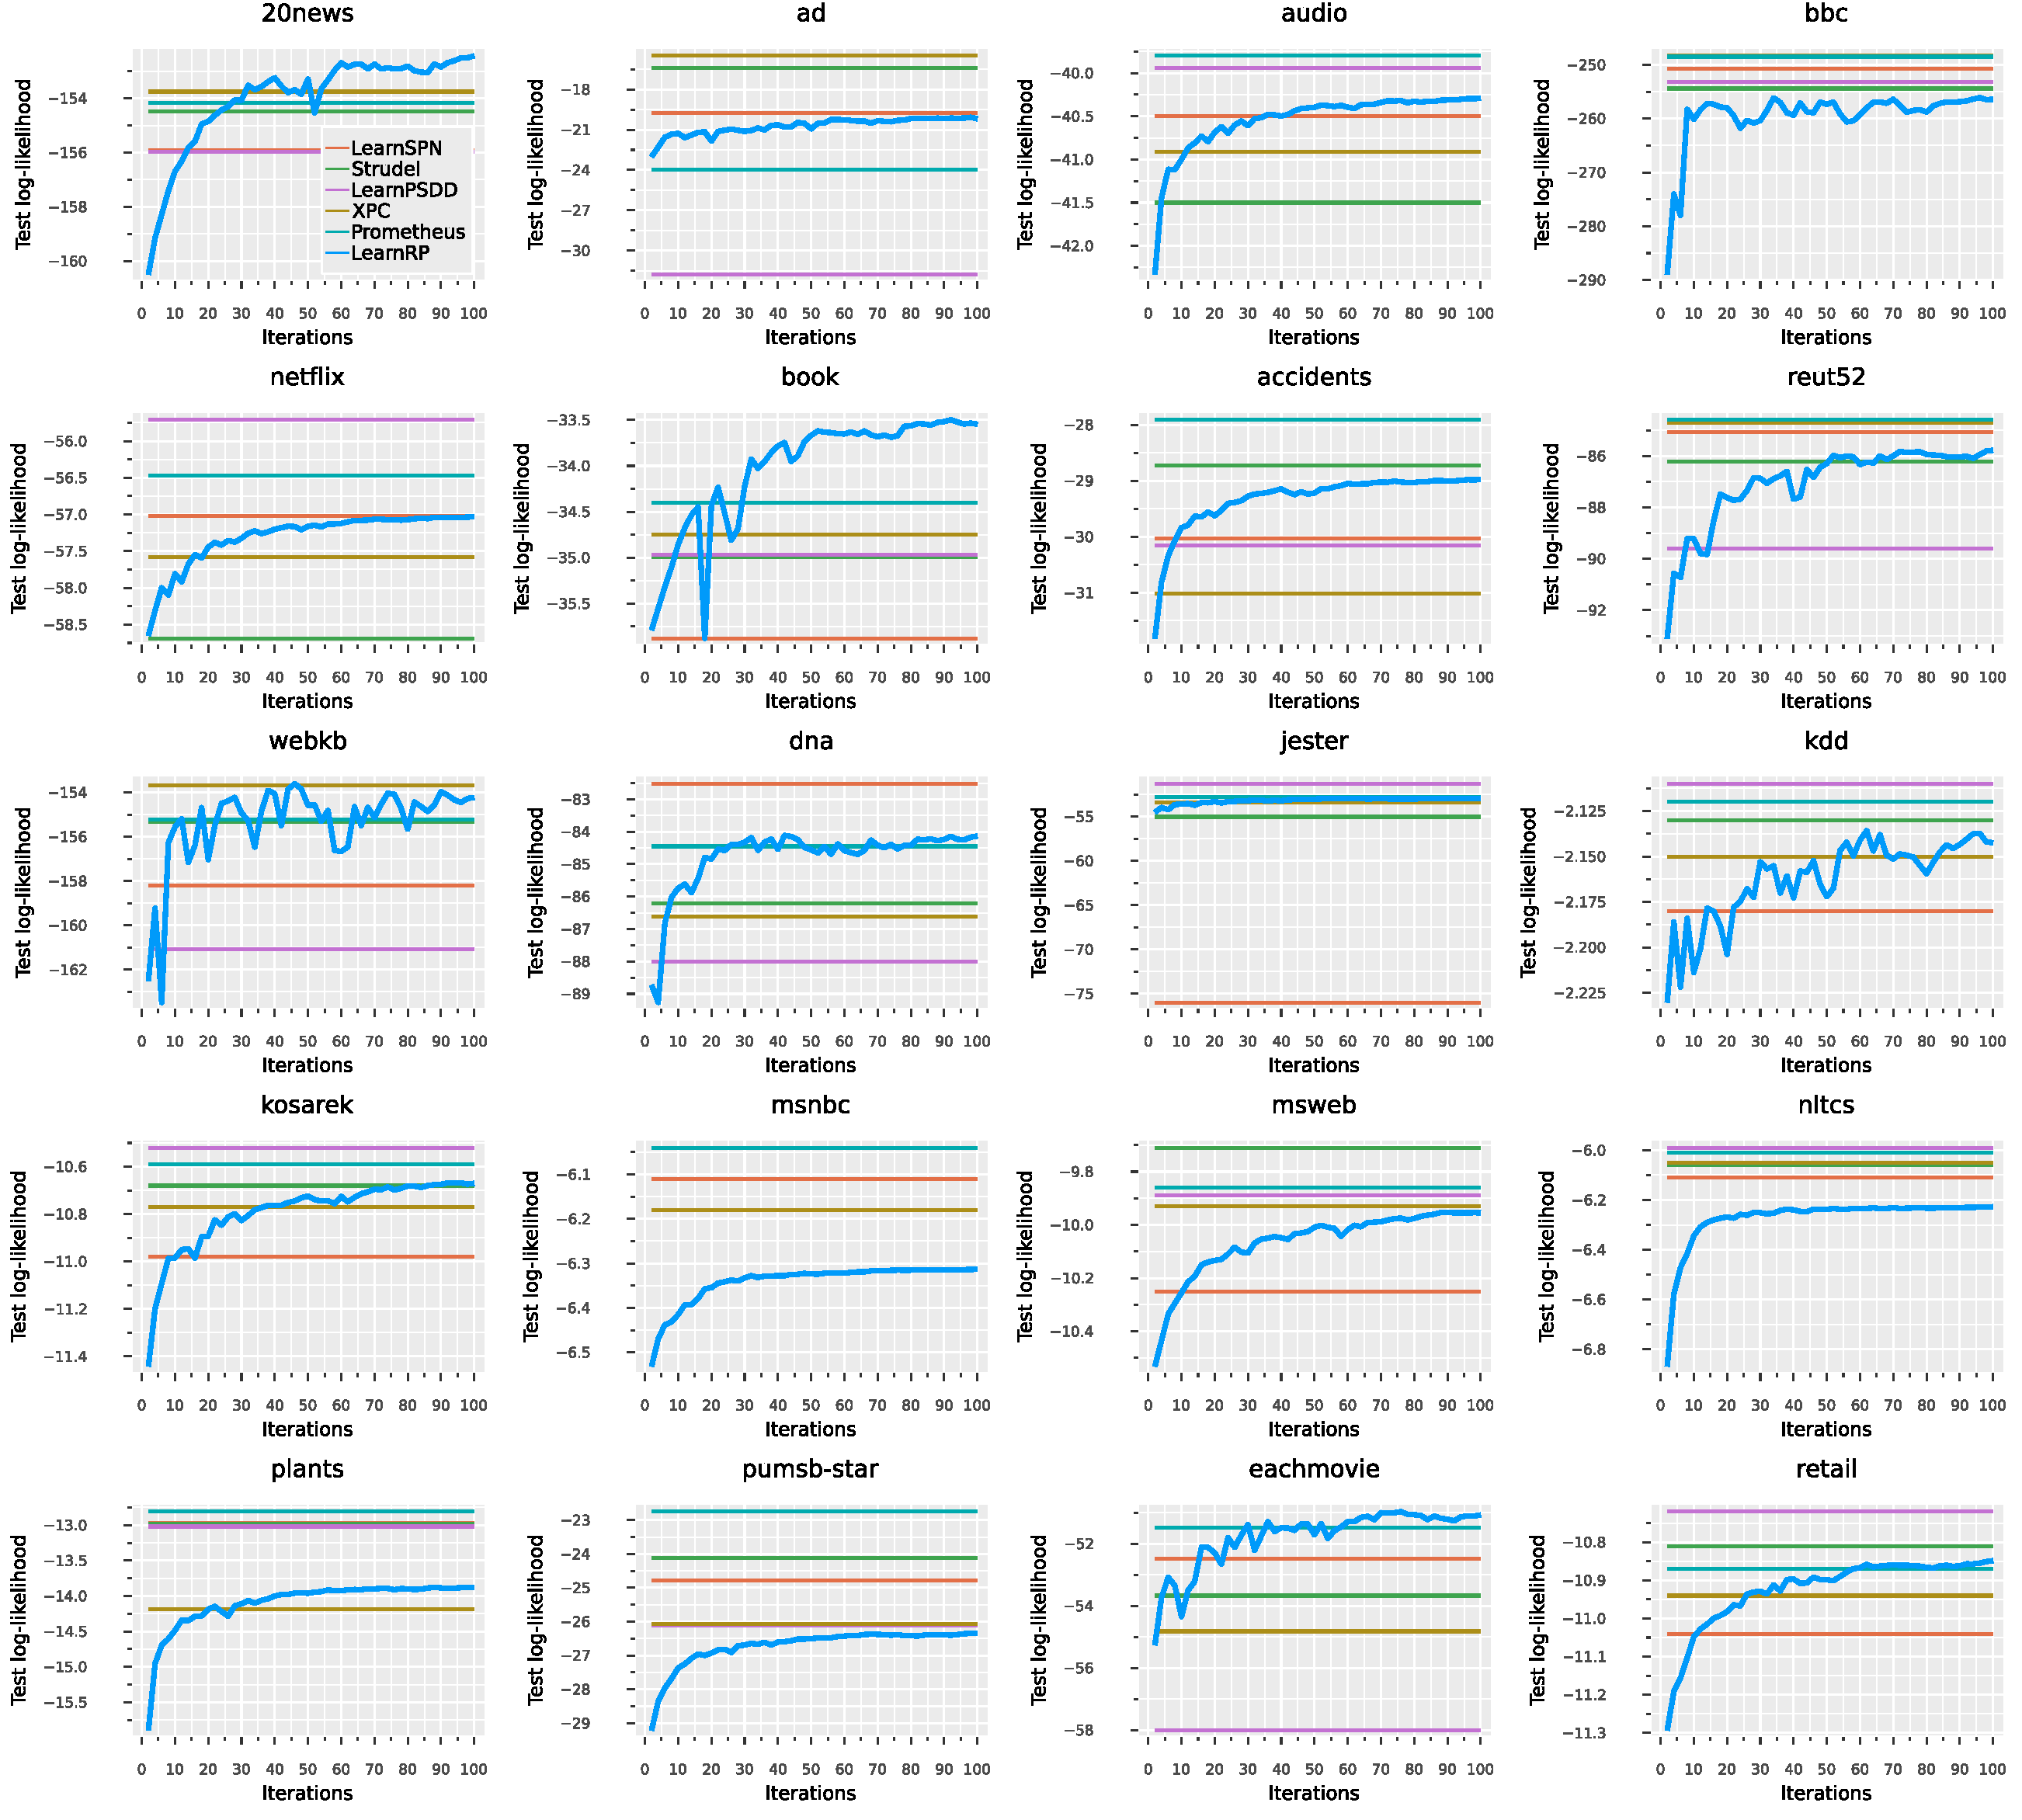
\includegraphics[width=\textwidth]{bins/all.pdf}
  \caption{Test log-likelihood performance of \textproc{LearnRP} shown as the curve in
    \protect\tikz\protect\fill[baseline=0.5ex,fill=jplots1] (0,0) rectangle (0.5,-0.1); under
    different iterations of minibatch EM. Each horizontal line shows the performance of a different
    competitor: \protect\tikz\protect\fill[baseline=0.5ex,fill=jplots2] (0,0) rectangle (0.5,-0.1);
    for \textproc{LearnSPN}, \protect\tikz\protect\fill[baseline=0.5ex,fill=jplots3] (0,0)
    rectangle (0.5,-0.1); for \textproc{Strudel},
    \protect\tikz\protect\fill[baseline=0.5ex,fill=jplots4] (0,0) rectangle (0.5,-0.1); for
    \textproc{LearnPSDD}, \protect\tikz\protect\fill[baseline=0.5ex,fill=jplots5] (0,0) rectangle
    (0.5,-0.1); for \textproc{XPC} and finally
    \protect\tikz\protect\fill[baseline=0.5ex,fill=jplots6] (0,0) rectangle (0.5,-0.1); for
    \textproc{Prometheus}}
  \label{fig:learnrp-curves}
\end{figure}

As a superficial ablation study of the impact of random projections on the parameterization of
probabilistic circuits, we verify and compare the performance of \textproc{LearnRP} under random
weights without modifying the structure. To be more precise, for each of the structures generated
in \Cref{fig:learnrp-curves}, we completely randomize all sum node weights without altering the PC
structure by uniformly sampling numbers in the $\left[0,1\right]\subset\mathbb{R}$ interval,
setting these as weights, and then normalizing sum edges such that the sum of all weights equal to
one. Once all weights have been randomized this way, we retrain with minibatch EM for 100
iterations. \Cref{fig:learnrp-rand-curves} shows the test log-likelihood curves for this random
initialization. We found that using the proportions of the random projection splits as sum weights
provided a better initial parameterization compared to random weight initialization, with the
former consistently achieving better final performance after 100 minibatch EM iterations. Notably,
in both the \textproc{ad} and \textproc{bbc} datasets, initializing weights as random severely
crippled the EM algorithm, causing it to be stuck at very low quality local maxima.

\begin{figure}[t]
  \centering
  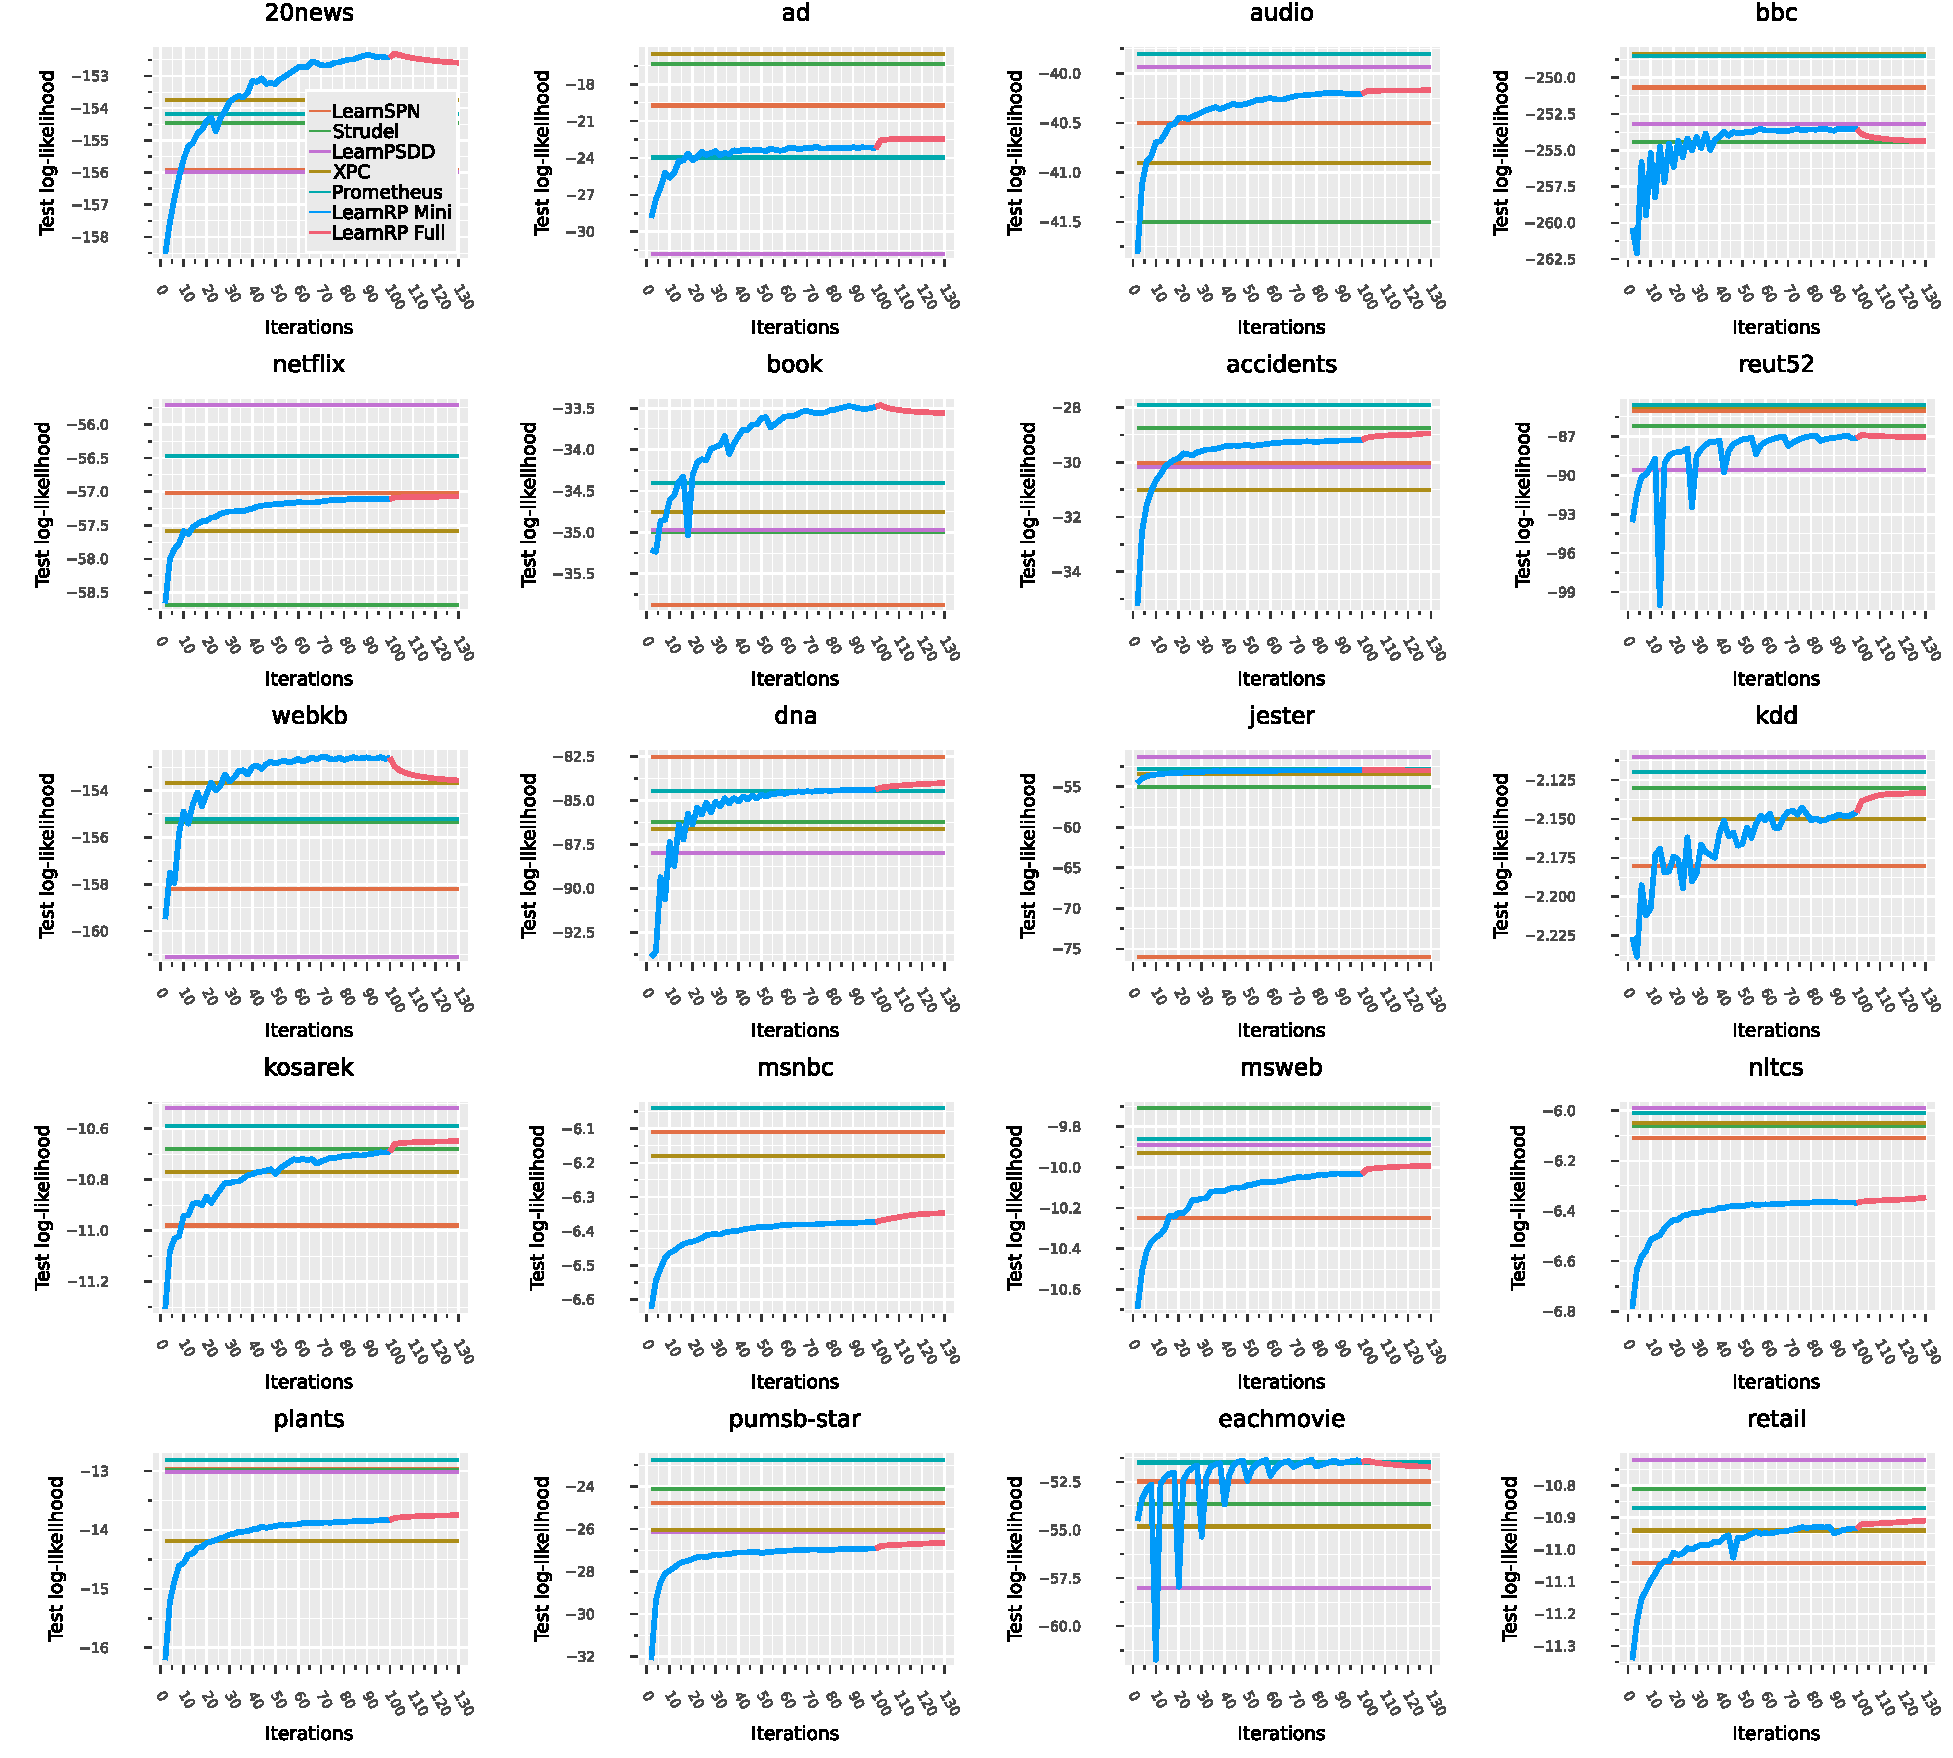
\includegraphics[width=\textwidth]{bins/all_rand.pdf}
  \caption{Test log-likelihood curve, shown in
    \protect\tikz\protect\fill[baseline=0.5ex,fill=jplots1] (0,0) rectangle (0.5,-0.1);, of
    \textproc{LearnRP} with randomized weights under different iterations of minibatch EM. Each
    horizontal line shows the performance of a different competitor:
    \protect\tikz\protect\fill[baseline=0.5ex,fill=jplots2] (0,0) rectangle (0.5,-0.1); for
    \textproc{LearnSPN}, \protect\tikz\protect\fill[baseline=0.5ex,fill=jplots3] (0,0) rectangle
    (0.5,-0.1); for \textproc{Strudel}, \protect\tikz\protect\fill[baseline=0.5ex,fill=jplots4]
    (0,0) rectangle (0.5,-0.1); for \textproc{LearnPSDD},
    \protect\tikz\protect\fill[baseline=0.5ex,fill=jplots5] (0,0) rectangle (0.5,-0.1); for
    \textproc{XPC} and finally \protect\tikz\protect\fill[baseline=0.5ex,fill=jplots6] (0,0)
    rectangle (0.5,-0.1); for
    \textproc{Prometheus}}
  \label{fig:learnrp-rand-curves}
\end{figure}

\begin{sidewaystable}[ph!]
  \resizebox{\textheight}{!}{
  \begin{tabular}{c|ccccc|ccccc}
    \hline
    \textbf{Dataset} & \textbf{\textproc{LearnSPN}} & \textbf{\textproc{Strudel}} &
    \textbf{\textproc{LearnPSDD}} & \textbf{\textproc{XPC}} & \textbf{\textproc{Prometheus}} &
    \textbf{\textproc{LearnRP}-F} & \textbf{\textproc{LearnRP}-100} & \textbf{\textproc{LearnRP}-30} &
    \textbf{\textproc{LearnRP}-20} & \textbf{\textproc{LearnRP}-10}\\
    \hline
    \textsc{accidents } & -30.03 & $|$-28.73$|$ & -30.16 & -31.02 & \textbf{-27.91} & \underline{-28.65} & -28.87 & -29.38 & -29.58 & -29.99\\
    \textsc{ad        } & -19.73 & \underline{-16.38} & -31.78 & \textbf{-15.50} & -23.96 & $|$-19.20$|$ & -20.32 & -21.42 & -21.44 & -21.94\\
    \textsc{audio     } & -40.50 & -41.50 & \underline{-39.94} & -40.91 & \textbf{-39.80} & $|$-40.18$|$ & -40.23 & -40.46 & -40.63 & -40.94\\
    \textsc{bbc       } & $|$-250.68$|$ & -254.41 & -253.19 & \textbf{-248.34} & \underline{-248.50} & -254.97 & -255.55 & -262.35 & -257.67 & -262.39\\
    \textsc{netflix   } & $|$-57.02$|$ & -58.69 & \textbf{-55.71} & -57.58 & \underline{-56.47} & -57.07 & -57.05 & -57.29 & -57.48 & -57.66\\
    \textsc{book      } & -35.88 & -34.99 & -34.97 & -34.75 & -34.40 & \underline{-33.57} & \textbf{-33.52} & -34.34 & $|$-34.24$|$ & -34.73\\
    \textsc{20-newsgrp} & -155.92 & -154.47 & -155.97 & $|$-153.75$|$ & -154.17 & \underline{-152.78} & \textbf{-152.76} & -154.32 & -155.03 & -156.26\\
    \textsc{reuters-52} & $|$-85.06$|$ & -86.22 & -89.61 & \underline{-84.70} & \textbf{-84.59} & -85.73 & -85.47 & -87.41 & -87.05 & -89.26\\
    \textsc{webkb     } & -158.20 & -155.33 & -161.09 & \underline{-153.67} & -155.21 & -154.43 & \textbf{-152.60} & -154.83 & $|$-154.33$|$ & -158.01\\
    \textsc{dna       } & \textbf{-82.52} & -86.22 & -88.01 & -86.61 & -84.45 & \underline{-83.03} & $|$-83.85$|$ & -84.77 & -84.98 & -85.40\\
    \textsc{jester    } & -75.98 & -55.03 & \textbf{-51.29} & -53.43 & \underline{-52.80} & -52.92 & $|$-52.89$|$ & -53.23 & -53.22 & -53.54\\
    \textsc{kdd       } & -2.18 & $|$-2.13$|$ & \textbf{-2.11} & -2.15 & \underline{-2.12} & $|$-2.13$|$ & -2.14 & -2.17 & -2.16 & -2.20\\
    \textsc{kosarek   } & -10.98 & -10.68 & \textbf{-10.52} & -10.77 & \underline{-10.59} & $|$-10.65$|$ & -10.67 & -10.79 & -10.86 & -11.00\\
    \textsc{msnbc     } & \underline{-6.11} & \textbf{-6.04} & \textbf{-6.04} & $|$-6.18$|$ & \textbf{-6.04} & -6.31 & -6.36 & -6.40 & -6.41 & -6.44\\
    \textsc{msweb     } & -10.25 & \textbf{-9.71} & -9.89 & -9.93 & $|$-9.86$|$ & \underline{-9.85} & -9.97 & -10.06 & -10.21 & -10.27\\
    \textsc{nltcs     } & -6.11 & -6.06 & \textbf{-5.99} & $|$-6.05$|$ & \underline{-6.01} & -6.35 & -6.23 & -6.25 & -6.27 & -6.32\\
    \textsc{plants    } & \underline{-12.97} & $|$-12.98$|$ & -13.02 & -14.19 & \textbf{-12.81} & -13.68 & -14.00 & -14.26 & -14.40 & -14.70\\
    \textsc{pumsb-star} & $|$-24.78$|$ & \underline{-24.12} & -26.12 & -26.06 & \textbf{-22.75} & -25.88 & -26.19 & -26.36 & -26.54 & -27.17\\
    \textsc{eachmovie } & -52.48 & -53.67 & -58.01 & -54.82 & $|$-51.49$|$ & \underline{-51.37} & \textbf{-51.06} & -51.55 & -52.86 & -52.21\\
    \textsc{retail    } & -11.04 & \underline{-10.81} & \textbf{-10.72} & -10.94 & -10.87 & $|$-10.85$|$ & -10.86 & -10.93 & -10.97 & -11.04\\
    \hline
    \multirow{2}{*}[-0.15em]{\textbf{Avg. Rank}} & $6.08\pm 3.03$ & $5.28\pm 2.97$ & $5.20\pm 3.86$ & $5.55\pm 2.76$ & \textbf{2.90}$\bm{\pm}$\textbf{2.07} & \underline{$3.83\pm 1.98$} & $|4.15\pm 2.03|$ & $6.35\pm 1.50$ & $6.95\pm 1.70$ & $8.72\pm 1.50$ \\
                                                 & $4.80\pm 1.91$ & $4.22\pm 1.81$ & $|4.05\pm 2.56|$ & $4.60\pm 1.93$ & \textbf{2.55}$\bm{\pm}$\textbf{1.43} & \underline{$3.62\pm 1.56$} & $4.15\pm 2.03$ \\
    \hline
  \end{tabular}
  }
  %[
    %-30.03   -28.73   -30.16   -31.02   -27.91   -30.18   -29.66   -29.17   -28.71  ;
    %-19.73   -16.38   -31.78   -15.50   -23.96   -22.51   -20.87   -20.37   -19.09  ;
    %-40.50   -41.50   -39.94   -40.91   -39.80   -41.05   -40.66   -40.68   -40.16  ;
    %-250.68  -254.41  -253.19  -248.34  -248.50  -259.17  -260.32  -254.09  -255.16 ;
    %-57.02   -58.69   -55.71   -57.58   -56.47   -59.91   -60.06   -57.60   -56.97  ;
    %-35.88   -34.99   -34.97   -34.75   -34.40   -36.15   -34.45   -33.95   -33.51  ;
    %-155.92  -154.47  -155.97  -153.75  -154.17  -158.10  -156.74  -154.35  -152.94 ;
    %-85.06   -86.22   -89.61   -84.70   -84.59   -91.61   -87.73   -86.62   -85.56  ;
    %-158.20  -155.33  -161.09  -153.67  -155.21  -156.40  -155.70  -156.40  -154.33 ;
    %-82.52   -86.22   -88.01   -86.61   -84.45   -86.55   -85.30   -85.61   -85.12  ;
    %-75.98   -55.03   -51.29   -53.43   -52.80   -53.67   -53.28   -53.13   -52.97  ;
    %-2.18    -2.13    -2.11    -2.15    -2.12    -2.20    -2.19    -2.15    -2.13   ;
    %-10.98   -10.68   -10.52   -10.77   -10.59   -10.97   -10.86   -10.85   -10.61  ;
    %-6.11    -6.04    -6.04    -6.18    -6.04    -6.39    -6.42    -6.39    -6.34   ;
    %-10.25   -9.71    -9.89    -9.93    -9.86    -10.23   -10.17   -10.10   -9.89   ;
    %-6.11    -6.06    -5.99    -6.05    -6.01    -6.30    -6.29    -6.37    -6.22   ;
    %-12.97   -12.98   -13.02   -14.19   -12.81   -14.76   -14.33   -14.26   -13.80  ;
    %-24.78   -24.12   -26.12   -26.06   -22.75   -27.14   -26.78   -26.75   -26.45  ;
    %-52.48   -53.67   -58.01   -54.82   -51.49   -52.68   -52.34   -51.43   -51.46  ;
    %-11.04   -10.81   -10.72   -10.94   -10.87   -11.08   -10.98   -10.95   -10.83  ;
  %]
  \caption{Performance of \textproc{LearnRP} in log-likelihood against state-of-the-art competitors
    in the twenty binary datasets for density estimation. Entries in \textbf{\textup{bold}}
    correspond to best performance, \underline{\textup{underlined}} entries are second best, and
    $|$\textup{barred}$|$ entries are third place. The last two rows refer to the average ranking
    of each algorithm across all datasets; the first compares rankings of all variants of
    \textproc{LearnRP} against competitors, while the last only compares \textproc{LearnRP}-F
    against the state-of-the-art.}
  \label{tab:binary}
\end{sidewaystable}

\Cref{tab:bintime} shows average running time for each learning algorithm to construct a
\emph{single} circuit for each dataset. Note that the performance reported in \Cref{tab:binary} for
\textproc{Strudel}, \textproc{LearnPSDD} and \textproc{XPC} correspond to ensemble results, meaning
that in all but \textproc{Strudel} (where a shared-structure mixture was learned) one has to
multiply the averages in \Cref{tab:bintime} with the number of components in the ensemble to get a
better picture of the speed difference. We note how, despite having competitive performance,
\textproc{LearnRP}-100 is orders of magnitude faster compared to \textproc{LearnSPN},
\textproc{Strudel} and \textproc{LearnPSDD}. When put against \textproc{XPC}, we note that
\textproc{LearnRP}-100 is consistently slower, albeit with better overall log-likelihood
performance as evidenced in \Cref{tab:binary}. Further, running 30 iterations of full EM boosted
performance considerably, although at the cost of having an overall learning time comparable to
more sophisticated algorithms. We also bring attention to the fact that, even though our EM
implementation makes use of CPU parallelization, there is much room for improvement, such as
bringing most of the computations to the GPU.

\Cref{tab:binsize} shows circuit sizes for each learning algorithm. All except for
\textproc{LearnSPN} are reported as in their original works to better reflect the log-likelihood
results shown in \Cref{tab:binary}. Because \citet{gens13} do not report circuit sizes, we report
values from our own runs. We do not show circuit sizes for \textproc{Prometheus} since we could not
find the source code and \citet{jaini18a} do not report circuit sizes.

\begin{table}[t]
  \resizebox{\textwidth}{!}{
  \begin{tabular}{c|cccc|ccccc}
    \hline
    \textbf{Dataset} & \textbf{\textproc{LearnSPN}} & \textbf{\textproc{Strudel}} &
    \textbf{\textproc{LearnPSDD}} & \textbf{\textproc{XPC}} & \textbf{\textproc{LearnRP}-F} &
    \textbf{\textproc{LearnRP}-100} & \textbf{\textproc{LearnRP}-30} &
    \textbf{\textproc{LearnRP}-20} & \textbf{\textproc{LearnRP}-10}\\
    \hline
    \textsc{nltcs}     & 7m   & 3m  & 6m    & 17s   & 3m19s & 15s    & 5s     & 3s     & 2s    \\
    \textsc{plants}    & 50m  & 41m & 26m   & 1m3s  & 26m   & 2m7s   & 41s    & 28s    & 15s   \\
    \textsc{audio}     & 2h   & 33m & 51m   & 1m58s & 37m   & 4m3s   & 1m16s  & 52s    & 28s   \\
    \textsc{jester}    & 52m  & 24m & 37m   & 1m20s & 29m   & 4m48s  & 1m29s  & 1m1s   & 31s   \\
    \textsc{netflix}   & 1h   & 14m & 33m   & 2m8s  & 46m   & 4m36s  & 1m28s  & 1m     & 32s   \\
    \textsc{accidents} & 47m  & 20m & 41m   & 1m47s & 33m   & 4m     & 1m20s  & 55s    & 31s   \\
    \textsc{book}      & >3h  & 8m  & 1h22m & 2m26s & 2h    & 25m13s & 7m55s  & 5m10s  & 2m43s \\
    \textsc{dna}       & >3h  & >3h & >3h   & 17s   & 11m   & 7m38s  & 2m20s  & 1m33s  & 49s   \\
    \hline
  \end{tabular}
  }
  \caption{Learning time benchmark for a single circuit of \textproc{LearnSPN}, \textproc{Strudel},
    \textproc{LearnPSDD}, \textproc{XPC} and \textproc{LearnRP}.}
  \label{tab:bintime}
\end{table}

\begin{table}[t]
  \resizebox{\textwidth}{!}{
  \begin{tabular}{c|cccc|ccccc}
    \hline
    \textbf{Dataset} & \textbf{\textproc{LearnSPN}} & \textbf{\textproc{Strudel}} &
    \textbf{\textproc{LearnPSDD}} & \textbf{\textproc{XPC}} &
    \textbf{\textproc{LearnRP}-F} & \textbf{\textproc{LearnRP}-100} & \textbf{\textproc{LearnRP}-30} &
    \textbf{\textproc{LearnRP}-20} & \textbf{\textproc{LearnRP}-10}\\
    \hline
    \textsc{accidents } & 32708   & 75363   & 8418  & 11921   &  18619 &   19086 &  19053 &  18498 &  18555 \\
    \textsc{ad        } & 40901   & 13152   & 12238 & 22093   & 100429 &   99807 &  98949 & 101471 & 100435 \\
    \textsc{audio     } & 50130   & 55675   & 18208 & 29317   &  19233 &   19463 &  19467 &  19249 &  19357 \\
    \textsc{bbc       } & 39389   & 29532   & 12335 & 14578   & 232199 &  234295 & 233743 & 230965 & 232541 \\
    \textsc{netflix   } & 36286   & 27173   & 10997 & 39868   &  21731 &   21675 &  21715 &  21719 &  21731 \\
    \textsc{book      } & 51493   & 54839   & 10978 & 13678   & 118811 &  119847 & 119491 & 118427 & 119511 \\
    \textsc{20-newsgrp} & 119060  & 58749   & 15793 & 65881   & 532657 &  534801 & 531615 & 536115 & 536709 \\
    \textsc{reuters-52} & 155191  & 36343   & 10410 & 36440   & 321594 &  320201 & 322981 & 320715 & 321095 \\
    \textsc{webkb     } & 223847  & 25406   & 11033 & 17122   & 251801 &  256322 & 256033 & 254797 & 256713 \\
    \textsc{dna       } & 12180   & 17507   & 3068  & 2616    &  37607 &   37399 &  37423 &  37515 &  37741 \\
    \textsc{jester    } & 25076   & 27713   & 11322 & 20273   &  23275 &   23111 &  23239 &  23363 &  23219 \\
    \textsc{kdd       } & 8755    & 6572    & 2915  & 13040   &   5251 &    5299 &   5353 &   5399 &   5265 \\
    \textsc{kosarek   } & 19512   & 37583   & 7173  & 20938   &  34013 &   33379 &  33167 &  33157 &  32865 \\
    \textsc{msnbc     } & 11606   & 20795   & 5465  & 4887    &    785 &     789 &    781 &    777 &    785 \\
    \textsc{msweb     } & 10743   & 2347    & 6581  & 12135   &  51239 &   51015 &  51911 &  51197 &  51009 \\
    \textsc{nltcs     } & 1855    & 4373    & 1304  & 4401    &    531 &     515 &    519 &    535 &    523 \\
    \textsc{plants    } & 36596   & 119194  & 11583 & 13960   &  10443 &   10711 &  10759 &  10779 &  10213 \\
    \textsc{pumsb-star} & 26206   & 108876  & 8298  & 8866    &  32332 &   30401 &  32102 &  31429 &  31856 \\
    \textsc{eachmovie } & 54184   & 123996  & 20648 & 21369   &  77839 &   80189 &  80073 &  78237 &  81705 \\
    \textsc{retail    } & 2158    & 3979    & 2989  & 6651    &  25578 &   24686 &  25081 &  25174 &  24844 \\
    \hline
  \end{tabular}
  }
  \caption{Circuit size (in the number of nodes) comparison between \textproc{LearnRP} and the
    state-of-the-art in the twenty binary datasets for density estimation.}
  \label{tab:binsize}
\end{table}

Overall, we found \textproc{LearnRP} to be competitive against the state-of-the-art, often
reaching second or first place in the case of \textproc{LearnRP}-F and \textproc{LearnRP}-100. As
expected for such a simple learning algorithm, it was hardly the best, although even under few EM
iterations it was capable of producing somewhat competitive models. Arguably, \textproc{LearnRP}'s
strengths come from its speed, learning circuits via minibatch EM in a fraction of the time when
compared to \textproc{LearnSPN}, \textproc{Strudel} and \textproc{LearnPSDD}. Perhaps the more
direct competitor of \textproc{LearnRP} in terms of scalability is \textproc{XPC}, showing the
strengths of \randclass{}-type learners when it comes to speed. Recall from \Cref{sec:xpcs},
however that \textproc{XPC} requires an extensive grid search on the hyperparameters, while the
performance of \textproc{LearnRP} mainly depends on how much time one is willing to spend to
fine-tune weights with parameter learning. Notably, we found that \textproc{LearnRP} performs worse
on data with fewer variables (e.g.\ \textsc{nltcs}, \textsc{msnbc}, \textsc{kdd}) and better on
data with more variables (e.g.\ \textsc{20-newsgrp}, \textsc{book}, \textsc{webkb}), which is
perhaps correlated with the smaller, and respectively larger, circuits from \Cref{tab:binsize}.

\subsection{Continuous data}
\label{sec:continuous}

\begin{table}[t]
  \resizebox{\textwidth}{!}{
  \begin{tabular}{cc|ccccccc|cc}
    \hline
    \textbf{Dataset} & \textbf{Vars} & \textbf{SRBMs} & \textbf{oSLRAU} & \textbf{GBMMs} & \textbf{iGMMs} &
    \textbf{GMMs} & \textbf{\textproc{Prometheus}} & \textbf{iSPTs} & \textbf{\textproc{LearnRP}} &
    \textbf{Size} \\
    \hline
    \textsc{abalone}    & 8  & -2.28  & $|$-0.94$|$  & -1.17  & ---   & \textbf{-0.59}   & \underline{-0.85}   & ---   & -6.13  & 317   \\
    \textsc{ca}         & 22 & -4.95  & \underline{21.19}  & $|$3.42$|$   & ---   & -1.08   & \textbf{27.82}   & ---   & -5.84  & 2765  \\
    \textsc{quake}      & 4  & -2.38  & \underline{-1.21}  & -3.76  & ---   & \textbf{-0.58}   & $|$-1.50$|$   & ---   & -3.76  & 79    \\
    \textsc{sensorless} & 48 & -26.91 & \underline{60.72}  & $|$8.56$|$   & ---   & -1.39   & \textbf{62.03}   & ---   & -38.46 & 12589 \\
    \textsc{banknote}   & 4  & -2.76  & \underline{-1.39}  & -4.64  & ---   & \textbf{-1.05}   & $|$-1.96$|$   & ---   & -6.06  & 79    \\
    \textsc{flowsize}   & 3  & -0.79  & \underline{15.32}  & $|$5.72$|$   & ---   & -36.50  & \textbf{18.03}   & ---   & 2.20   & 49    \\
    \textsc{kinematics} & 8  & \textbf{-5.55}  & -11.13 & -11.20 & ---   & \underline{-6.11}   & -11.12  & ---   & $|$-11.02$|$ & 319   \\
    \textsc{iris}       & 4  & ---    & ---    & ---    & -3.94 & \textbf{0.20}    & \underline{-1.06}   & -3.74 & $|$-3.47$|$  & 79    \\
    \textsc{oldfaith}   & 2  & ---    & ---    & ---    & $|$-1.73$|$ & -2.09   & \textbf{-1.48}   & \underline{-1.70} & -4.33  & 19    \\
    \textsc{chemdiabet} & 3  & ---    & ---    & ---    & -3.02 & \textbf{-0.58}   & \underline{-2.59}   & $|$-2.88$|$ & -18.68 & 48    \\
    \hline
  \end{tabular}
  }
  \caption{Performance of \textproc{LearnRP} in log-likelihood against state-of-the-art competitors
    in ten continuous datasets for density estimation and function approximation. Entries in
    \textbf{\textup{bold}} correspond to best performance, \underline{\textup{underlined}} entries
    are second best, and $|$\textup{barred}$|$ entries are third place. Last column shows size (in
    the number of nodes) of circuits learned with \textproc{LearnRP}.}
  \label{tab:cont}
\end{table}

\Cref{tab:cont} shows results for continuous data. Note that some entries are positive since the
log-likelihood of continuous variables can be positive. As previously mentioned, reported
performance of SRBMs, oSLRAU, GBMMs, and \textproc{Prometheus} come from \citet{jaini18a}, while
iGMM and iSPT reports come from \citet{trapp16}. For comparison, we trained standard GMMs with 5
Gaussians as components and diagonal covariances through the \texttt{GaussianMixtures.jl}
library\footnote{Available at \url{https://github.com/davidavdav/GaussianMixtures.jl}.}. Component
centers were initialized with $k$-means, with GMM weights and Gaussian variances learned through
EM. Because the evaluated continuous datasets were small in size, we only show results for
\textproc{LearnRP} under 100 iterations of EM. We also do not run full EM after the batch variant
as we found performance to degrade after doing so. When constructing the circuit with
\textproc{LearnRP}, we use mixtures of three Gaussians as input nodes. We learn both sum weights
and input GMMs through EM. The last column of \Cref{tab:cont} shows the circuit sizes of
\textproc{LearnRP}.

We found that \textproc{LearnRP} behaves extremely poorly on continuous datasets. This could
possibly be due to the smaller number of variables in these datasets (as evidenced by the reduced
circuit sizes in \Cref{tab:cont}'s last column), causing \textproc{LearnRP} to produce very small
models. We also point to the fact that full EM was degrading the performance of \textproc{LearnRP}
which is a possible indication that our EM implementation may suffer from numerical issues and/or
perhaps that the learned circuit is overfitting the training data.

\section{Summarizing \textproc{LearnRP}}

By taking inspiration from the decision tree literature, we have proposed in this chapter an
efficient and effective way of constructing probabilistic circuits through random projections. Our
approach generates random smooth and structured decomposable PCs in a manner similar to
\textproc{LearnSPN}. Contrastively to \textproc{LearnSPN}, however, instead of running clustering
algorithms to divide data instances as a means to learn sum nodes, we resort to a faster and
simpler alternative: we randomly sample a hyperplane in order to linearly divide the data in two.
This, coupled with the fact that products are derived from the partitioning induced by a vtree,
accelerates learning to the point that, even after optimizing weights through minibatch EM, our
technique is orders of magnitude faster than most popular PC learning algorithms.

We summarize \textproc{LearnRP} by adding it as a new entry in \Cref{tab:learning-all}. We note
that, although the number of projection trials $k$ is set as a parameter, we do not classify it as
a hyperparameter, as the quality of partitions only increases with a higher valued $k$.

\begin{sidewaystable}
  \resizebox{\textheight}{!}{
    \begin{tabular}{c|clcc|cccc|ccc|c}
    \hline
    \textbf{Name} & \textbf{Class} & \multicolumn{1}{c}{\textbf{Time Complexity}} & \textbf{\# hyperparams}
    & \textbf{Accepts logic?} & \textbf{Smooth?} & \textbf{Dec?} & \textbf{Det?} & \textbf{Str Dec?} &
    \textbf{$\mathbf{\{0,1\}}$?} & $\mathbb{N}$\textbf{?} & $\mathbb{R}$\textbf{?} & \textbf{Reference}\\
    \hline
    \textproc{LearnSPN} & \divclass{} & $
    \begin{cases}
      \bigo\left(nkmc\right) & \text{, if sum}\\
      \bigo\left(nm^3\right) & \text{, if product}
    \end{cases}
    $ & $\geq 2$ & \xmark & \cmark & \cmark & \xmark & \xmark & \cmark & \cmark & \cmark & \Cref{sec:learnspn}\\
    \textproc{ID-SPN} & \divclass{} & $
    \begin{cases}
      \bigo\left(nkmc\right) & \text{, if sum}\\
      \bigo\left(nm^3\right) & \text{, if product}\\
      \bigo\left(ic(rn+m)\right)  & \text{, if input}
    \end{cases}
    $ & $\geq 2+3$ & \xmark & \cmark & \cmark & \xmark & \xmark & \cmark & \cmark & \xmark & \Cref{sec:idspn}\\
    \textproc{Prometheus} & \divclass{} & $
    \begin{cases}
      \bigo\left(nkmc\right) & \text{, if sum}\\
      \bigo\left(m(\log m)^2\right) & \text{, if product}
    \end{cases}
    $ & $\geq 1$ & \xmark & \cmark & \cmark & \xmark & \xmark & \cmark & \cmark & \cmark & \Cref{sec:prometheus}\\
    \hline
    \textproc{LearnPSDD} & \incrclass{} & $
    \begin{cases}
      \bigo\left(m^2\right) & \text{, top-down vtree}\\
      \bigo\left(m^4\right) & \text{, bottom-up vtree}\\
      \bigo\left(i|\mathcal{C}|^2\right) & \text{, circuit structure}
    \end{cases}
    $ & $1$ & \cmark & \cmark & \cmark & \cmark & \cmark & \cmark & \xmark & \xmark & \Cref{sec:learnpsdd}\\
    \textproc{Strudel} & \incrclass{} & $
    \begin{cases}
      \bigo\left(m^2 n\right) & \text{, CLT + vtree}\\
      \bigo\left(i\left(|\mathcal{C}|n+m^2\right)\right) & \text{, circuit structure}
    \end{cases}
    $ & $1$ & \cmark & \cmark & \cmark & \cmark & \cmark & \cmark & \xmark & \xmark & \Cref{sec:strudel}\\
    \hline
    & & & & & & & & & & & & \\
    \textproc{RAT-SPN} & \randclass{} & $\phantom{\{}\bigo\left(rd(s+l)\right)$ & $4$ & \xmark & \cmark & \cmark
                       & \xmark & \xmark & \cmark & \cmark & \cmark & \Cref{sec:ratspn}\\
    & & & & & & & & & & & & \\
    \textproc{XPC} & \randclass{} & $\phantom{\{}\bigo\left(i(t+kn)+ikm^2n\right)$ & $3$ & \xmark &\cmark & \cmark
                   & \cmark & \cmark & \cmark & \xmark & \xmark & \Cref{sec:xpcs}\\
    & & & & & & & & & & & & \\
    \hline
    \textproc{SamplePSDD} & \randclass{} & $
    \begin{cases}
      \bigo\left(m\right) & \text{, random vtree}\\
      \bigo\left(kc\log c+\log_2^2 k\right) & \text{, per call}
    \end{cases}
    $ & $1$ & \cmark & \cmark & \cmark & \cmark & \cmark & \cmark & \xmark & \xmark & \Cref{ch:logical}\\
    \textproc{LearnRP} & \randclass{} & $
    \begin{cases}
      \bigo\left(m^2\right) & \text{, top-down vtree}\\
      \bigo\left(m^4\right) & \text{, bottom-up vtree}\\
      \bigo\left(knm\right) & \text{, per call}
    \end{cases}
    $ & $0$ & \xmark & \cmark & \cmark & \xmark & \cmark & \cmark & \cmark & \cmark & \Cref{ch:data}\\
    \hline
  \end{tabular}
  }
  \caption{Summary of all structure learning algorithms for probabilistic circuits described so far.}
  \label{tab:learning-all}
\end{sidewaystable}
